\documentclass[spanish]{article}
\usepackage[utf8]{inputenc}
\usepackage[spanish]{babel}
\usepackage{graphicx}
\usepackage{verbatim}
\usepackage{moreverb}
\usepackage{amsmath}
\usepackage{amsfonts}
\usepackage{amssymb}
\usepackage{fancybox}
\usepackage{float}
\usepackage{fancyvrb}
\usepackage{color}
\usepackage{listings}
\usepackage{url}



\usepackage{esvect}
\usepackage{breqn}
\usepackage{mathtools}
\usepackage{placeins}
\usepackage{tabu}

\usepackage{hyperref} % for references to link.
\usepackage{cite} % for cite references.

\definecolor{dkgreen}{rgb}{0,0.6,0}
\definecolor{gray}{rgb}{0.5,0.5,0.5}
\definecolor{mauve}{rgb}{0.58,0,0.82}


% Defines Code Snippets properties
\lstset{frame=tb,
  language=Octave,
  aboveskip=3mm,
  belowskip=3mm,
  showstringspaces=true,
  columns=flexible,
  basicstyle={\small\ttfamily},
  numbers=left,
  numberstyle=\color{gray},
  keywordstyle=\color{blue},
  commentstyle=\color{gray},
  stringstyle=\color{dkgreen},
  breaklines=true,
  breakatwhitespace=true,
  tabsize=4,
  captionpos=b % captions to bottom
}






\selectlanguage{spanish}


% UTF-8, font and 'pdf copy & paste fix'
\usepackage{tgtermes}
\usepackage[T1]{fontenc}
\usepackage[utf8]{inputenc}
\input{glyphtounicode}

% Changes lstlistings caption to "Código"
\renewcommand{\lstlistingname}{Algoritmo}
\renewcommand\spanishtablename{Tabla}


\renewcommand{\shorthandsspanish}{}


\newcommand{\HRule}{\rule{\linewidth}{0.5mm}}


\newcommand\abs[1]{\left|#1\right|}
\newcommand\norm[1]{\left\lVert#1\right\rVert}

\newcommand{\proj}[2][]{\textit{proj}_{#1} \thinspace #2}



\begin{document}


    % Carátula
    \begin{titlepage}
        \begin{center}
            
            % Logo ITBA
            
\includegraphics[scale=0.40]{./logo_itba.png}\\[1cm]

            % Materia, Nro TP, Cuatrimestre y Año
            \textsc{\LARGE Métodos Numéricos Avanzados}\\[1.5cm]
            \textsc{\Large Trabajo Práctico 1}\\[0.5cm]
            \textsc{\Large Segundo Cuatrimestre 2016}\\[0.5cm]

            % Título
            \HRule \\[0.4cm]
            { \huge \bfseries Random Sparse Matrix}\\[0.4cm]
            \HRule \\[1.5cm]
            
            % Autores
            \Large Autores: \\ [0.25cm]
            \begin{tabular}{l @{\ \ -\ \ }l}
                \emph{\Large José Carlos Noriega Defferrari} & \Large 51231\\[0.2cm]
                \emph{\Large Juan Marcos Bellini} & \Large 52056\\[0.2cm]
                \emph{\Large Franco Cesar Prudhomme} & \Large 54263\\[0.2cm]
                \emph{\Large Luis Ignacio Marzoratti} & \Large 55449\\[0.2cm]
                \emph{\Large Raffael Rudolf Düll} & \Large 58598\\[0.2cm]
            \end{tabular}

            % Keywords
            \renewcommand{\abstractname}{Palabras clave:}
            
            \begin{abstract}
                \centering
                \textbf{Random Sparse Matrix, Matriz rala, Autovalores, QR, Gram-Schmidt, MVMRAN, MATRAN}
            \end{abstract}

            \vfill
            % La fecha queda abajo.
            {\large 30 de Septiembre de 2016}

        \end{center}
    \end{titlepage}


    \fvset{frame=single}
    \clearpage
    
    % Índice
    \tableofcontents
    \clearpage

    % Resumen
    \section{Resumen}
        \par Las matrices dispersas son aquellas cuyos elementos son, en su mayoría, iguales a cero. Conceptualmente, son matrices que representan sistemas con bajo acoplamiento entre sus elementos. El foco principal del trabajo se centra en la manipulación de dichas matrices, y el cálculo de sus autovalores.


    \section{Introducción}

        \par El almacenamiento y procesamiento de matrices de gran tamaño por medio de una computadora, utilizando los métodos tradicionales, requiere una gran cantidad de recursos (tiempo y memoria). Es por ello que se han diseñado algoritmos específicos para matrices dispersas (o también llamadas, matrices ralas)\footnote{\url{https://es.wikipedia.org/wiki/Matriz_dispersa}}.
        \par El siguiente informe trata acerca de la generación de matrices dispersas aleatorias (\textit{Random Sparse Matrix}, en inglés), y el cálculo de sus autovalores. A continuación, se detallarán los algoritmos utilizados, las dificultades encontradas, y las decisiones tomadas para solucionar dichos problemas. Luego se mostrarán los resultados obtenidos, y se elaboraran conclusiones en base a ellos.

    \section{Metodología}

        \subsection{Implementación}
        
            \par La implementación de los métodos fue realizada en su totalidad en el lenguaje de programación \textit{Octave}, utilizando la plataforma \textit{GNU Octave}\footnote{\url{https://www.gnu.org/software/octave/}}, debido a su gran eficiencia en cuanto a la manipulación de matrices, además de su facilidad y simplicidad de uso.
            \par El cálculo de autovalores fue llevado a cabo por el algoritmo QR\footnote{\url{https://es.wikipedia.org/wiki/Algoritmo_QR}}, el cual se basa en la descomposición QR de una matriz. Dicha descomposición fue efectuada a través de tres métodos distintos: Gram-Schmidt, Gram-Schmidt modificado y Rotaciones de Givens.

        \subsection{Construcción de la matriz dispersa aleatoria (RSM)}
        
            \par La construcción de matrices ralas aleatorias fue realizada por un programa que recibe dos parámetros, $N$ y $NZR$. El primero representa la dimensión de dicha matriz. Cabe destacar que el resultado es una matriz cuadrada de $N\times N$. El segundo parámetro, $NZR$, indica la cantidad de valores distintos de $0$ (cero) por columna.
            
            \par Para que el programa funcione correctamente, el valor de $N$ debe ser mayor o igual al valor de $NZR$. De hecho, cuanto menor sea la cantidad de valores distintos de $0$ por columna, mayor sera la dispersidad de la matriz resultante.
            
            \par A continuación se presenta el algoritmo implementado:
            
            \begin{lstlisting}[caption = Construcción de matrices dispersas aleatorias.]
function RSMMatrix = generateRSM(N, NZR)
	RSMMatrix = zeros(N);
	for columnIndex = 1 : N
		for i = 1 : NZR
			do
				rowIndex = ceil(rand() * N);
			until (RSMMatrix(rowIndex, columnIndex) == 0)
			do
				RSMMatrix(rowIndex, columnIndex) = rand() * 2 - 1;
			until (RSMMatrix(rowIndex, columnIndex) != 0)
		end
	end
end
            \end{lstlisting}
            
            \par El método genera una matriz cuadrada de $N\times N$ inicializada con todos sus valores en $0$. Luego recorre dicha matriz de izquierda a derecha generando tantos valores aleatorios – en filas aleatorias – como el valor de $NZR$. Dichos valores aleatorios pertenecen al conjunto $[-1, 1]$.
           
            \par Se puede ver en la linea 7 que el programa verifica que una posición ya ocupada por un valor no nulo sea ignorada, volviendo a seleccionar una fila al azar. Además, también se comprueba que el valor aleatorio a asignar en la posición elegida no sea $0$ – linea 10.


        \subsection{Descomposición QR}
        
        \par Se han implementado tres métodos distintos para obtener la descomposición $QR$ de matrices. De esta manera se pudo realizar un \textit{benchmark} entre los mismos. Cada método recibe como parámetro una matriz cualquiera – llamada matriz $A$ – y retorna las matrices $Q$ y $R$ en un vector resultado.
            
        \subsubsection{Descomposición QR por Gram-Schmidt}
        
            \par El primer algoritmo implementado es la descomposición $QR$ a través del método de ortogonalización de Gram-Schmidt. Para el mismo, se toman las columnas de la matriz $A$  como vectores que se quieren ortonormalizar, y se aplica el método de Gram-Schmidt. Los vectores resultantes forman las columnas de la matriz $Q$. Dicha matriz tiene la propiedad de ser ortogonal, por lo que el cálculo de la matriz $R$ puede efectuarse como $R = Q^T\ A$.
            \par Matemáticamente, el método se puede resumir en las siguientes ecuaciones\footnote{Apuntes de cátedra: Descomposición QR, sección 2}:
            
            
            \begin{equation}
                \vec{q}_{1} = \dfrac{\vec{a}_{1}}{\norm{\vec{a}_{1}}}
            \end{equation}
            
            \begin{align}
                \vec{w}_{i} = \vec{a}_{i} - \sum_{j = 1}^{i - 1}{\proj[\vec{w}_{j}]{\vec{a}_{i}}} \;\;\;\;con\: i\: \in \{2,3, ..., N\}
            \end{align}
            
            \begin{equation}
                \vec{q}_{i} = \dfrac{\vec{w}_{i}}{\norm{\vec{w}_{1}}}
            \end{equation}
            
            siendo $\vec{a_{i}}$ la i-ésima columna de $A$, y $\vec{q_{i}}$ la i-ésima columna de $Q$. Una vez obtenida ésta última, $R$ se puede calcular como se ha dicho anteriormente: $R = Q^T\ A$.
           
            \vspace{5mm}
           
            \par A continuación se encuentra la implementación del algoritmo:
            
            \begin{lstlisting}[caption = Descomposición $QR$ por Gram-Schmidt.]
function [Q R] = gramSchmidtQRDecomposition(matrix)
	Q = matrix;
	for i = 1 : columns(matrix)
		for j = 1 : (i - 1)
			scalarProduct = matrix(:, i)' * Q(:, j);
			Q(:, i) -= scalarProduct * Q(:, j);
		end
		if (norm(Q(:,i)) < 0.00001)
			Q(:,i) = zeros(rows(Q),1);
		else
			Q(:, i) /= norm(Q(:, i));
		end
	end
	R = Q' * matrix;
end
            \end{lstlisting}
            
            \par El programa copia la matriz $A$ de entrada en la matriz $Q$, utilizando esta última como contenedora de los vectores ortonormalizados. En la i-ésima iteración externa se toma un nuevo vector columna de $A$ – llamado $\vec{a_{i}}$ – y se lo ortonormaliza respecto de los $i - 1$ vectores ya ortonormales contenidos en las primeras $i - 1$ columnas de $Q$ ($\vec{q}_{1}, \vec{q}_{2}, ... , \vec{q}_{i-1}$). En la j-ésima iteración interna se calcula la proyección de $\vec{a_{i}}$ sobre $\vec{q_{j}}$.  
            \par Como se puede ver en la linea 11, en el i-ésimo paso se normaliza el vector $\vec{q_{i}}$ obtenido, en caso de no ser el vector nulo. De esta manera, la siguiente iteración puede calcular las proyecciones de manera más simple (no tiene que dividir el vector $\vec{q_{j}}$ por el cuadrado de su norma). En caso de que el vector sea el nulo (o dicho de otra manera, en caso de que la norma del vector sea $0$), se lo deja como esta. Para no trabajar con valores pequeños, se le asigna una columna de $0$s a la matriz $Q$.
            
            \par Sin embargo, este método tiene una gran desventaja. Produce vectores de norma pequeña, lo cual puede llevar a grandes errores numéricos, que luego son arrastrados y amplificados en cada paso del algoritmo. Es por ello que se ha implementado una modificación al proceso de ortogonalización de Gram-Schmidt.

            
        \subsubsection{Descomposición QR por Gram-Schmidt modificado}
        
        
            \par El problema del método clásico de Gram-Schmidt es la gran cantidad de errores numéricos que se pueden producir al ser utilizado en una computadora. El resultado es un conjunto de vectores que no son del todo ortogonales. Debido a esto, se le hace una modificación al proceso de Gram-Schmidt. En este caso, las matrices $Q$ y $R$ se construyen a medida que avanza el algoritmo. Además, se modifica – en caso de no haberla resguardado – la matriz $A$. A continuación una breve explicación matemática\footnote{Apuntes de cátedra: Descomposición QR, sección 2.1}.
            
            \par Por cómo se define la factorización $QR$, cada elemento de $A$ se puede expresar según el siguiente producto de matrices:
            
            \begin{equation}
                a_{ij} = 
                    \begin{bmatrix}
                            q_{i 1} & q_{i 2} & \cdots & q_{i n}
                    \end{bmatrix}
                    \begin{bmatrix}
                        r_{1 j}\\
                        r_{2 j}\\
                        \vdots\\
                        r_{n j}
                    \end{bmatrix}
                    = \sum_{k = 1}^{n} q_{i k} r_{k j}
            \end{equation}
            
            siendo $n$ la cantidad de columnas de $Q$,y de filas de $R$, $q_{i j}$ el elemento en la fila $i$ y la columna $j$ de $Q$, y $r_{i j}$ es el elemento en la fila $i$ y la columna $j$ de $R$. Tener en cuenta que las matrices $A$ y $Q$ son matrices de $n\times m$. La matriz $R$ es de $n\times n$, con la particularidad de ser triangular superior.
            \par Continuando con el razonamiento, la j-ésima columna de la matriz $A$ – o $\vec{a}_{j}$ – se puede expresar segun:
            
            \begin{equation}
                \vec{a}_{j} =
                \arraycolsep=1.4pt\def\arraystretch{1.5}
                \begin{bmatrix}
                        
                        \sum_{k = 1}^{n} q_{1 k} r_{k j}\\
                        \sum_{k = 1}^{n} q_{2 k} r_{k j}\\
                        \vdots\\
                        \sum_{k = 1}^{n} q_{m k} r_{k j}\\
                    \end{bmatrix}
            \end{equation}
            
            A su vez, la matriz $A$ se la puede expresar como:
            
            \begin{equation}
                A = 
                \arraycolsep=1.4pt\def\arraystretch{0.9}
                \begin{bmatrix}
                    \vec{a}_{1} & \vec{a}_{2} & \cdots & \vec{a}_{n} 
                \end{bmatrix}
                =
                \arraycolsep=1.4pt\def\arraystretch{1.5}
                \begin{bmatrix}
                    \sum_{k = 1}^{n} q_{1 k} r_{k 1} & \sum_{k = 1}^{n} q_{1 k} r_{k 2} & \cdots & \sum_{k = 1}^{n} q_{1 k} r_{k n} \\
                    \sum_{k = 1}^{n} q_{2 k} r_{k 1} & \sum_{k = 1}^{n} q_{2 k} r_{k 2} & \cdots & \sum_{k = 1}^{n} q_{2 k} r_{k n} \\
                    \vdots & \vdots & \ddots & \vdots\\
                    \sum_{k = 1}^{n} q_{m k} r_{k 1} & \sum_{k = 1}^{n} q_{m k} r_{k 2} & \cdots & \sum_{k = 1}^{n} q_{m k} r_{k n}
                \end{bmatrix}
            \end{equation}
            
            
            \par Sin embargo, por cómo opera el algoritmo de ortogonalización de Gram-Schmidt, es evidente que las primeras $k$ columnas de $A$ se puede expresar en función de las primeras $k$ columnas de $Q$. Expresado según la sintaxis de \textit{Octave}:
            
            \begin{equation}
                \begin{split}
                    A(:,1:k) &= 
                    \arraycolsep=1.4pt\def\arraystretch{0.9}
                    \begin{bmatrix}
                        \vec{a}_{1} & \vec{a}_{2} & \cdots & \vec{a}_{k}
                    \end{bmatrix}
                    \\
                    &=
                    \arraycolsep=1.4pt\def\arraystretch{1.5}
                    \begin{bmatrix}
                        \sum_{l = 1}^{k} Q(1,l) R(l,1) & \cdots & \sum_{l = 1}^{n} Q(1,l) R(l,k) \\
                        \sum_{l = 1}^{k} Q(2,l) R(l,1) & \cdots & \sum_{l = 1}^{n} Q(2,l) R(l,2) \\
                        \vdots & \ddots & \vdots\\
                        \sum_{l = 1}^{k} Q(m,l) R(l,1) & \cdots & \sum_{l = 1}^{n} Q(m,l) R(l,k)
                    \end{bmatrix}
                    \\
                    &= \sum_{l = 1}^{k} Q(:,l) R(l,:) = \sum_{l = 1}^{k} \vec{q}_{l} \vec{r}^{T}_{l}
                \end{split}
            \end{equation}
            
            Nótese que, para simplificar la notación en la ecuación (7), se piensa a la matriz $R$ de la siguiente manera:
            
            \begin{equation}
                R = 
                \begin{bmatrix}
                    \vec{r}^{T}_{1}\\
                    \vec{r}^{T}_{2}\\
                    \vdots\\
                    \vec{r}^{T}_{n}
                \end{bmatrix}
            \end{equation}
            
            En base a lo anterior, se puede definir una nueva matriz $A^{(k)} \in \mathbb{R}^{m \times (n - k + 1)}$ según:
            
            \begin{equation}
                A - \sum_{l = 1}^{k - 1} \vec{q}_{l} \vec{r}^{T}_{l} = \sum_{l = k}^{n} \vec{q}_{l} \vec{r}^{T}_{l} =
                \begin{bmatrix}
                    0 & A^{(k)}
                \end{bmatrix}
            \end{equation}
            
            Si se llama $\vec{x}$ a la primera columna de $A^{(k)}$, y $B$ a la matriz formado por el resto de las columna 
            (o sea, $A^{(k)} = \begin{bmatrix} \vec{x} & B\end{bmatrix}$), y se multiplica miembro a miembro por $\vec{q}^{T}_{k}$, se obtiene la siguiente ecuación:
            
            
            \begin{equation}
                \begin{split}
                    \vec{q}^{T}_{k} \sum_{l = k}^{n} \vec{q}_{l} \vec{r}^{T}_{l} 
                    &=
                    \sum_{l = k}^{n} \vec{q}^{T}_{k} \vec{q}_{l} \vec{r}^{T}_{l}
                    = \vec{r}^{T}_{k}
                    \\ 
                    &=
                    \vec{q}^{T}_{k} 
                    \begin{bmatrix}
                        0 & A^{(k)}
                    \end{bmatrix} 
                    = \vec{q}^{T}_{k}
                    \begin{bmatrix}
                        0 &\vec{x} & B
                    \end{bmatrix}
                    =
                    \begin{bmatrix}
                        0 & \vec{q}^{T}_{k} \vec{x} & \vec{q}^{T}_{k} B
                    \end{bmatrix}
                \end{split}
            \end{equation}
            
            Por lo tanto, se tiene que
            
            \begin{equation}
                \vec{r}^{T}_{k} = 
                \begin{bmatrix}
                    0 & \vec{q}^{T}_{k} \vec{x} & \vec{q}^{T}_{k} B
                \end{bmatrix}
            \end{equation}
             
                    
            Como $\vec{q}^{T}_{k}$ debe tener norma unitaria, entonces $\abs{R(k,k)} = \norm{\vec{q}^{T}_{k} \vec{x}}_{2}$. Por lo tanto, se pueden fijar las siguientes relaciones:
            
            \begin{equation}
                R(k,k) = \norm{\vec{x}}_{2}
            \end{equation}
            
            \begin{equation}
                \vec{q}_{k} = \dfrac{\vec{a}}{\norm{\vec{x}}_{2}} = \dfrac{\vec{x}}{R(k,k)}
            \end{equation}
            
            De esta forma, se puede calcular $A^{(k + 1)}$ como
            
            \begin{equation}
                A^{(k + 1)} = B - (\vec{q}_{k} \vec{r}^{T}_{k})(k + 1 : n)
            \end{equation}
            
            
             \vspace{5mm}
             
            \par Gracias a ésta última ecuación, la ecuación (14), se puede implementar el siguiente algoritmo.
            
            \begin{lstlisting}[caption = Descomposición $QR$ por Gram-Schmidt modificado]
function [Q R] = modifiedGramSchmidtQRDecomposition(matrix)
	Q = matrix;
	cols = columns(matrix);
	for i = 1 : cols
		R(i, i) = norm(matrix(:, i));
		Q(:, i) = matrix(:, i) / R(i, i);
		for j = i + 1 : cols
			R(i, j) =  matrix(:, j)' * Q(:, i);
			matrix(:, j) -=  R(i, j) * Q(:, i);
		end
	end
end
            \end{lstlisting}





        \subsubsection{Descomposición con rotaciones de Givens}
            
            \par Otra forma de calcular la descomposición $QR$ de una matriz $A$ es a través de matrices de rotación de Givens\footnote{Apuntes de cátedra: Descomposición QR, sección 4}. Una matriz de rotación tiene la siguiente forma:
            
            \begin{equation}
                G_{\theta} = 
                        \begin{bmatrix}
                            \cos{\theta} & \sin{\theta} \\
                            -\sin{\theta} & \cos{\theta}
                        \end{bmatrix}
            \end{equation}

            Estas matrices se pueden utilizar para anular elementos de una matriz cualquiera. 
            
            \paragraph{Matriz de Rotación de Givens} ~
            \par Sin perder generalidad, suponiendo que se quiere anular el elemento $a_{q p}$, con $p \text{ \textless } q$, de la matriz $A$, se genera la matriz $G$ de la siguiente manera:
            
            \begin{equation}
                G(k,k) = 
                    \begin{cases}
                        \cos{\theta}, & \text{si $k = p,q$}\\
                        1, & \text{en otro caso}
                    \end{cases}
            \end{equation}
            
            \begin{equation}
                G(k,k) = 
                    \begin{cases}
                        +\sin{\theta}, & \text{si $k = p$ y $l = q$}\\
                        -\sin{\theta}, & \text{si $k = 1$ y $l = p$}\\
                        0, & \text{en otros casos en que $k \neq l$}
                    \end{cases}
            \end{equation}
            
            
            Como se puede ver, $G$ se parece a la matriz identidad, difiriendo en las filas $p$ y $q$. A esta matriz se la llama matriz de rotación de Givens. Es una matriz ortogonal. Además, al pre-multiplicarla por la matriz $A$, solo afecta las filas $p$ y $q$ de ésta última. Llamando $c = \cos{\theta}$ y $s =\sin{\theta}$, se puede establecer la siguiente relación:
            
            
            \begin{equation}
                \begin{split}
                    G([p,q],[p,q]) A([p,q],[p,q])
                    &=
                        \begin{bmatrix}
                            c & s\\
                            -s & c
                        \end{bmatrix}
                        \begin{bmatrix}
                            A_{pp} & A_{pq}\\
                            A_{qp} & A_{qq}
                        \end{bmatrix}
                    \\
                    &=
                        \begin{bmatrix}
                            c A_{pp} + s A_{qp} & c A_{pq} + s A_{qq}\\
                            -s A_{pp} + c A_{qp} & -s A_{pq} + c A_{qq}
                        \end{bmatrix}
                \end{split}
            \end{equation}
            
            
            Se desea que se cumpla la siguiente condición:
            
            \begin{equation}
                -s A_{p p} + c A_{q p} = 0
            \end{equation}
            
            Para ello, basta con hacer
            
            \begin{equation}
                \tan{\theta} = \dfrac{s}{c} = \dfrac{A_{q p}}{A_{p p }}
            \end{equation}
            
            Sin embargo, no se necesita calcular el valor de $\theta$ para calcular $c$ y $s$. Definiendo $t = \tan{\theta}$:
            
            \begin{equation}
                \begin{split}
                    1 + t^{2} = 1 + \dfrac{s^{2}}{c^{2}} 
                    &= \dfrac{c^{2} + s^{2}}{c^{2}} = \dfrac{1}{c^{2}}\\
                    &\Rightarrow c = \dfrac{1}{\sqrt{1 + t^{2}}}, s = ct
                \end{split}
            \end{equation}
            
            También se podría definir:
            
            \begin{equation}
                z = \dfrac{1}{\tan{\theta}} = \dfrac{c}{s} = \dfrac{A_{p p}}{A_{q}{q}}
            \end{equation}
            
            En este caso, se procedería de la siguiente forma:
            
            \begin{equation}
                \begin{split}
                    1 + z^{2} = 1 + \dfrac{c^{2}}{s^{2}} 
                    &= \dfrac{s^{2} + c^{2}}{s^{2}} = \dfrac{1}{s^{2}}\\
                    &\Rightarrow s = \dfrac{1}{\sqrt{1 + z^{2}}}, c = sz
                \end{split}
            \end{equation}
            
            
            Según cuál sea el caso, conviene trabajar con la ecuación (21), o con la ecuación (23). Suponiendo que, por errores de redondeo, se trabaje con 
            
            \begin{equation}
                \hat{A}_{q p} = A_{q p} + \epsilon_{1}, \hat{A}_{p p} = A_{p p} + \epsilon_{2}
            \end{equation}
            
            con $\epsilon_{1}, \epsilon_{2} \geq 0$. Llamando $\hat{c}_{1}, \hat{s}_{1}$ a los valores obtenidos utilizando la ecuación (21) y las definiciones establecidas en la ecuación (24), se obtienen los siguientes resultados:
            
            \begin{equation}
                \hat{t} = \dfrac{\hat{A}_{q p}}{\hat{A}_{p p}} \approx t \left(1 + \dfrac{\epsilon_{1}}{\hat{A}_{q p}} - \dfrac{\epsilon_{2}}{\hat{A}_{p p}}\right)
            \end{equation}
            
            \begin{equation}
                \hat{c}_{1} = \dfrac{1}{\sqrt{1 + \hat{t}^{2}}} \approx c \left[1 + s^{2}\left( \dfrac{\epsilon_{1}}{\hat{A}_{q p}} - \dfrac{\epsilon_{2}}{\hat{A}_{p p}}\right)\right]
            \end{equation}
            
            \begin{equation}
                \hat{s}_{1} = \hat{c}_{1} \hat{t} \approx s \left[1 + s^{2}\left( \dfrac{\epsilon_{1}}{\hat{A}_{q p}} - \dfrac{\epsilon_{2}}{\hat{A}_{p p}}\right)\right]
            \end{equation}
            
            haciendo uso reiterado del desarrollo en serie de Taylor\footnote{\url{https://es.wikipedia.org/wiki/Serie_de_Taylor}} de primer orden, y la hipótesis de que $\abs{\epsilon_{i}} \ll 1, i \in \{1,2\}$. De manera similar, llamando $\hat{c}_{2}, \hat{s}_{2}$ a los valores obtenidos utilizando la ecuación (23) y las definiciones establecidas en la ecuación (24), y nuevamente haciendo uso reiterado del desarrollo en serie de Taylor de primer orden, se obtienen:
            
            
            \begin{equation}
                \hat{z} = \dfrac{\hat{A}_{p p}}{\hat{A}_{q p}} \approx z \left(1 + \dfrac{\epsilon_{2}}{\hat{A}_{p p}} - \dfrac{\epsilon_{1}}{\hat{A}_{q p}}\right)
            \end{equation}
            
            \begin{equation}
                \hat{s}_{2} = \dfrac{1}{\sqrt{1 + \hat{z}^{2}}} \approx s \left[1 + c^{2}\left( \dfrac{\epsilon_{2}}{\hat{A}_{p p}} - \dfrac{\epsilon_{1}}{\hat{A}_{q p}}\right)\right]
            \end{equation}
            
            \begin{equation}
                \hat{c}_{2} = \hat{s}_{2} \hat{z} \approx c \left[1 + c^{2}\left( \dfrac{\epsilon_{2}}{\hat{A}_{p p}} - \dfrac{\epsilon_{1}}{\hat{A}_{q p}}\right)\right]
            \end{equation}
            
            \par Tomando como ejemplo $s$, al comparar el error absoluto utilizando las ecuaciones (21) y (23):
            
            \begin{equation}
                \dfrac{\abs{\Delta s_{1}}}{\abs{\Delta s_{2}}} 
                = \dfrac{\abs{\hat{s}_{1} - s_{1}}}{\abs{\hat{s}_{2} - s_{2}}}
                \approx \dfrac{\abs{s}^{3} \abs{ \dfrac{\epsilon_{1}}{A_{q p}} - \dfrac{\epsilon_{2}}{A_{p p}}}}
                    {\abs{s} c^{2} \abs{ \dfrac{\epsilon_{2}}{A_{p p}} - \dfrac{\epsilon_{1}}{A_{q p}}}}
                = \dfrac{s^{2}}{c^{2}} = \left( \dfrac{A_{q p}}{A_{p p}} \right)^{2}
                \approx \left( \dfrac{\hat{A}_{q p}}{\hat{A}_{p p}} \right)^{2}
            \end{equation}
            
            se puede concluir que, si $\abs{\hat{A}_{q p}} \text{\textless} \abs{\hat{A}_{p p}}$, conviene utilizar la ecuación 21. En caso contrario, conviene la ecuación 23.
            
            \par Todo este razonamiento se puede resumir en el siguiente algoritmo:
            \begin{lstlisting}[caption = Cálculo de los elementos $c$ y $s$ de una matriz de rotación de Givens]
function [c s] = givensrotation(a, b)
    if (b == 0)
    c = 1;
    s = 0;
    else
        if (abs(b) > abs(a))
            r = a / b;
            s = 1 / sqrt(1 + r**2);
            c = s * r;
        else
            r = b / a;
            c = 1 / sqrt(1 + r**2);
            s = c * r;
        end
    end
end
            \end{lstlisting}
            
            \par Como se puede ver, el algoritmo recibe dos valores: $a$ y $b$. El primero de ellos, $a$, representa el valor $A_{p p}$. Por otro lado, $b$ representa $A_{q p}$. 
            
            
            \paragraph{Factorización QR utilizando matrices de rotación de Givens} ~
            \par Como se dijo al comienzo de esta sección, las matrices de rotación de Givens pueden ser utilizadas para calcular la descomposición $QR$ de una matriz $A$. Lo que de debe hacer es anular todos los elementos de la matriz por debajo de la diagonal principal utilizando rotaciones de Givens. A continuación se encuentra la implementación del algoritmo:
            

            \begin{lstlisting}[caption = Descomposición en $QR$ con rotaciones de Givens]
function [Q R] = givensRotationQRDecomposition(A)
    m = rows(A);
    Q = eye(m);
    R = A;

    for j = 1 : n
        for i = m : -1 : (j + 1)
            G = eye(m);
            [c, s] = givensrotation(R(i - 1, j), R(i, j));
            G([i - 1, i], [i - 1, i]) = [c - s; s c];
            R = G' * R;
            Q = Q * G;
        end
    end
end
            \end{lstlisting}
            
            \par Como se puede ver en el código, en la linea 9 se hace uso de la función definida en el algoritmo 4 de este documento.




        \subsection{Cálculo de autovalores}
        
            \par Para calcular los autovalores de la matriz se utilizó un método global de aproximación, utilizando las descomposiciones $QR$ mencionadas anteriormente. Se siguió un documento\footnote{\url{http://www.win.tue.nl/casa/meetings/seminar/previous/_abstract051109_files/presentation_full.pdf}} sobre técnicas iterativas para encontrar los autovalores, contemplando el hecho de que los mismos pudieran ser tanto valores reales como complejos.
            
            \par Se emplearon la técnica de corrimiento simple para acelerar la convergencia de los valores cuando los módulos de los autovalores están cerca el uno del otro, y la de corrimiento doble para contemplar los valores complejos.
            
            \par El método opera de la siguiente manera. Primero calcula la descomposición $QR$ de $A$, y luego obtiene una nueva matriz $A^{\prime} = R * Q$. Se tienen en cuenta los elementos de la diagonal para calcular los autovalores (siguiendo el algoritmo iterativo referenciado en la bibliografía), teniendo en cuenta si el autovalor es real o complejo.
            
            
        
            \begin{lstlisting}[caption = Implementación del método QR de obtención de autovalores]
function eigenvalues = calculateEigenvalues(A, error, decomposition)
    eigenvalues = [];
    n = columns(A);
    current = 0;
    do
        previousA = A;
        [Q R] = decomposition(A);
        A = R * Q;
        if (condition(error, A(n - current, n - current - 1), A(n - current - 1, n - current - 1), A(n - current, n - current)))
            eigenvalues(n - current, 1) = A(n - current, n - current);
            A = A(1:n - current - 1, 1:n - current - 1);
            current++;
        elseif (condition(error, A(n - current -1, n - current - 2), A(n - current - 1, n - current - 1), A(n - current - 2, n - current - 2)))
            [r1 r2] = getValues(A, n, current);
            eigenvalues(n - current - 1, 1) = r1;
            eigenvalues(n - current, 1) = r2;
            A = A(1:n - current - 2, 1:n - current - 2);
            current += 2;
        end
    until (current >= n - 2)
    
    if (current == n - 2)
        [r1 r2] = getValues(A, n, current);
        eigenvalues(n - current - 1, 1) = r1;
        eigenvalues(n - current, 1) = r2;
        A = A(1:n - current - 2, 1:n - current - 2);
    elseif (current == n - 1)
        eigenvalues(1) = A(1, 1);
    end
end
    
function bool = condition(error, value1, value2, value3)
    bool = abs(value1) < (error * (abs(value2) + abs(value3)));
end
    
function [r1 r2] = getValues(A, n, current)
    w = A(n - current - 1, n - current - 1);
    x = A(n - current - 1, n - current);
    y = A(n - current, n - current - 1);
    z = A(n - current, n - current);
    rootValues = roots([1 -(w+z) (w*z)-(x*y)]);
    r1 = rootValues(1);
    r2 = rootValues(2);
end
            \end{lstlisting}
        
    \section{Resultados y conclusiones}
    
    \par Se han realizado dos \textit{benchmarks} sobre los algoritmos implementados. El primero fue realizado sobre el método de obtención de autovalores de la matriz $A$ utilizando los tres algoritmos de cálculo de la factorización $QR$ de dicha matriz. Se evaluó el tiempo – en segundos – que le toma hacer el cálculo de los autovalores, en función del tamaño de la matriz de entrada. Se han utilizado matrices cuadradas de $n \times n$.
    
    \par Las pruebas se realizaron con una baja densidad de valores no nulos por columna (0.25), repitiendo el proceso 30 veces. De esta manera se puede obtener un promedio que se ajusta a la realidad. Los resultados – que se pueden observar en la figura 1 de este documento – muestran que el método de factorización $QR$ más rápido es el algoritmo de ortonormalización de Gram-Schmidt clásico. Luego sigue el método modificado de Gram-Schmidt. Por último, el algoritmo que más tiempo le lleva terminar es el de las rotaciones de Givens. El resultado es evidente. A mayor estabilidad numérica que posea el algoritmo, mayor costo computacional tiene. A la hora de seleccionar uno de ellos, el usuario debe analizar la situación, y elegir qué desea sacrificar: tiempo o precisión.
    
    \begin{figure}[H]
        \centering
        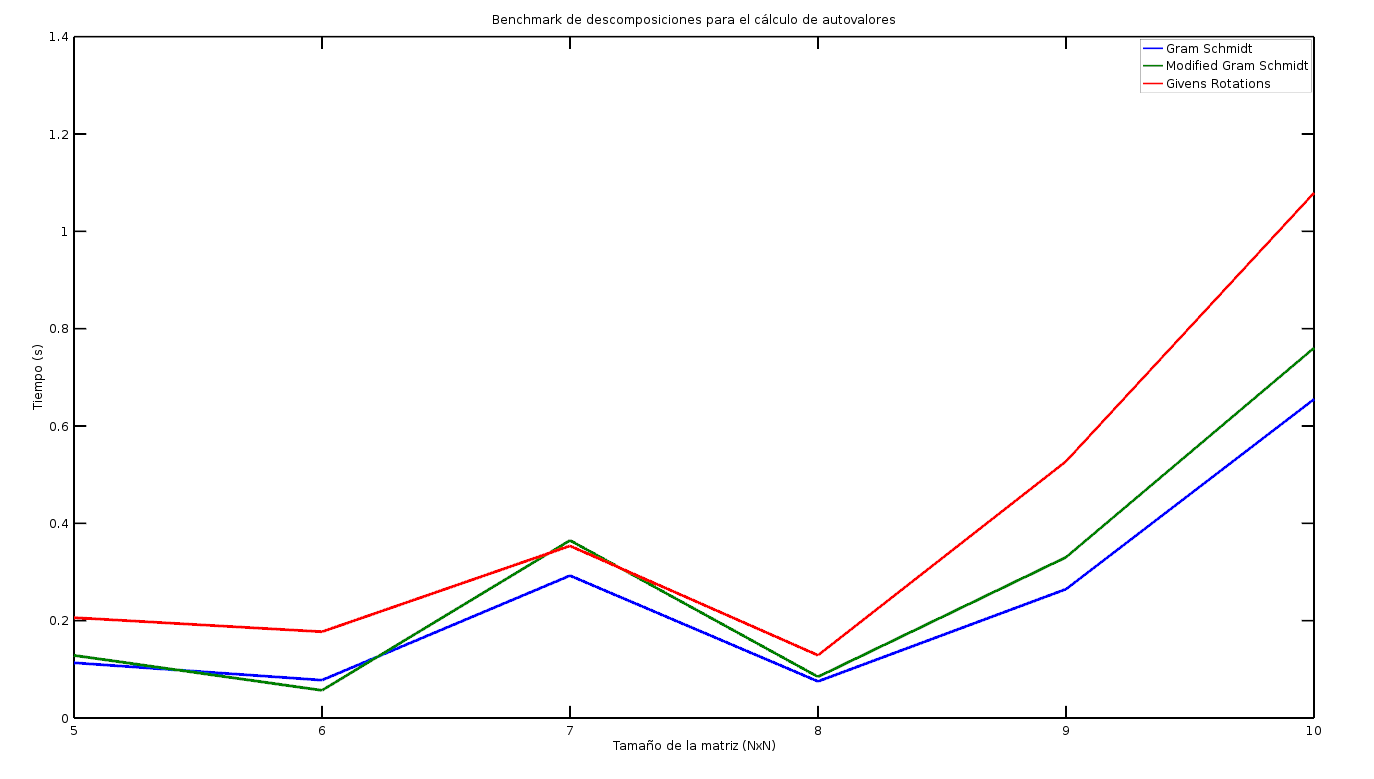
\includegraphics[scale=0.22]{./ben3.png}
        \caption{Resultados del \textit{benchmark} realizado al algoritmo de cálculo de autovalores}
    \end{figure}
    
    \vspace{5mm}
     
    \par El segundo \textit{benchmark} realizado fue sobre el método mostrado en el algoritmo 1 de de este documento. Se evaluó la función que genera matrices dispersas aleatorias. Para el mismo se mantuvo constante el valor $NZR$, logrando una densidad de valores no nulos por columna de 0.25, y variando el valor de $N$, para ver cuánto tiempo – nuevamente en segundos – tarda el programa en devolver la matriz. Los resultados se pueden ver en la figura 2.
    
    
    \begin{figure}[H]
        \centering
        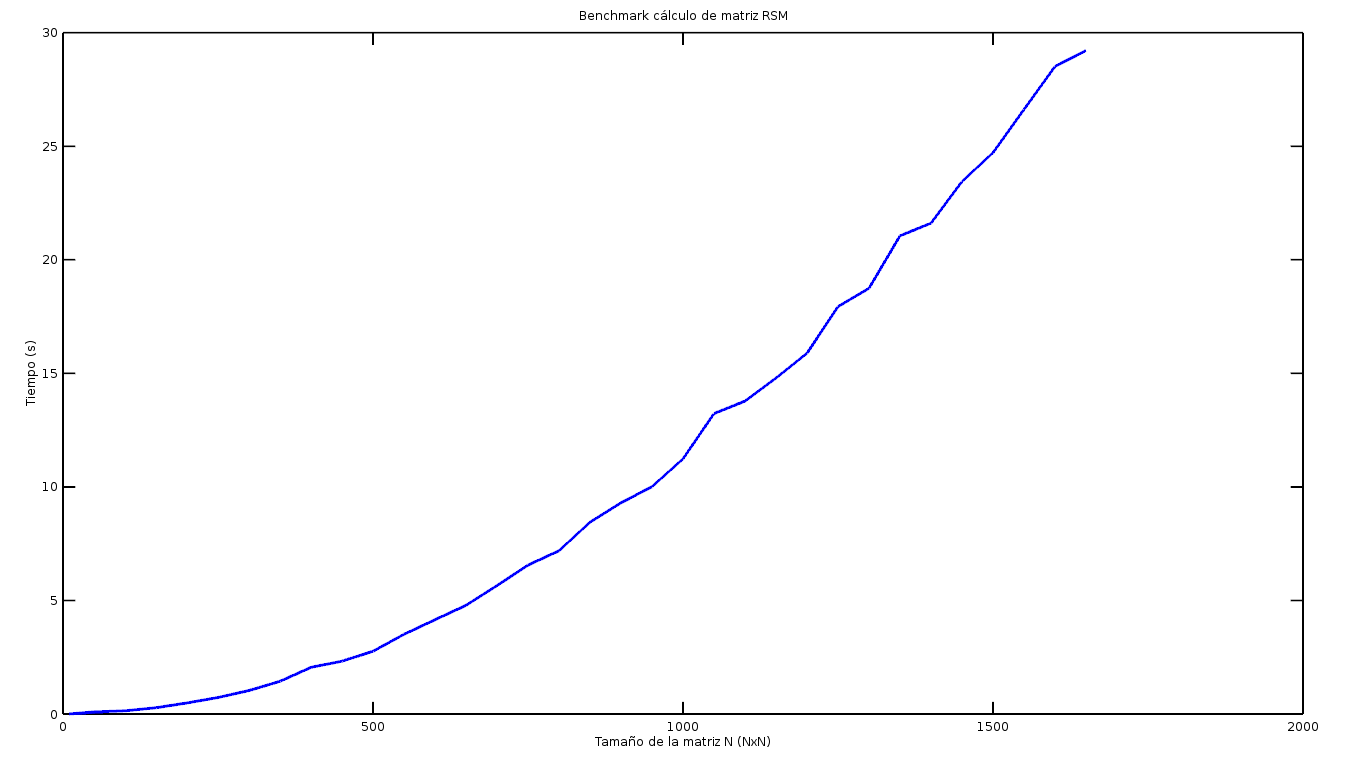
\includegraphics[scale=0.22]{./ben2.png}
        \caption{Resultados del \textit{benchmark} realizado al programa de generación de matrices dispersas aleatorias}
    \end{figure}
    
    
    \par Por último, tomando el método de descomposición $QR$ con el que mejor resultados se obtuvieron, se procedió a verificar el valor de $N$ máximo para el cual el programa retorna en un tiempo razonable. Los resultados se pueden observar en la tabla 1. Se puede notar que para valores de $N \text{\textless} 40$, el algoritmo tarda alrededor de $60 s$. También se puede observar que con valores entre $40$ y $60$, el tiempo es razonable, variando entre $1$ minuto y $5$ minutos. Sin embargo, con valores de $N \text{\textgreater} 60$, el programa se vuelve muy lento, creciendo dicho tiempo a medida que crece el valor de $N$.
    
    \begin{center}
        \begin{table}[H]
            \centering
            \begin{tabu}{|[1pt] l | l |[1pt]}
                \tabucline[1 pt]{-}
                $N$ &   Tiempo $\left[s\right]$     \\
                \tabucline[1 pt]{-} 
                10  &   5.32730                     \\ 
                15  &   0.72258                     \\ 
                20  &   3.95338                     \\ 
                25  &   16.42223                    \\ 
                30  &   16.62530                    \\                     
                35  &   20.04132                    \\ 
                40  &   73.99459                    \\ 
                45  &   51.05616                    \\ 
                50  &   120.50823                   \\ 
                55  &   221.21567                   \\ 
                60  &   391.32867                   \\ 
                65  &   540.01190                   \\ 
                70  &   892.09711                   \\ 
                \tabucline[1 pt]{-}
            \end{tabu}
            \caption{Tiempo de ejecución para obtener autovalores de matrices de $N \times N$ para distintos valores de N}
        \end{table}
            
    \end{center}
    
    \clearpage
    \section{Bibliografía}
    
        \begin{itemize}
    
        \item Introducción a Random Sparse Matrix: \url{http://www.staff.science.uu.nl/~bisse101/Book/PSC/psc4_7.pdf}
        
        \item Matrix Market MATRAN: \url{http://math.nist.gov/MatrixMarket/data/NEP/matran/matran.html}
        
        \item Técnicas iterativas para encontrar autovalores:  \url{http://www.win.tue.nl/casa/meetings/seminar/previous/_abstract051109_files/presentation_full.pdf}
        
        \item Wikipedia \url{https://www.wikipedia.org}
        
        \item Apuntes de cátedra: Descomposición QR
        
        \end{itemize}
    
\end{document}

